\documentclass[12pt]{article}

\usepackage[brazil]{babel}
\usepackage[utf8]{inputenc}
\usepackage{amsmath}
\usepackage{amsfonts}
\usepackage{amssymb}
\usepackage{indentfirst}
\usepackage{color}
\usepackage{mathrsfs}
\usepackage{pgfplots}
\usepackage{hyperref}
\usepackage{fancyhdr}


\fancypagestyle{plain}{%
	\fancyfoot{}%
	\fancyhead{}%
}
\fancyhead{}
\fancyhead[L]{\leftmark}
\fancyfoot{}
\fancyfoot[L]{{\footnotesize  COMPPET - Programa de Educação Tutorial}}
\fancyfoot[C]{\hspace{3.0cm}\thepage}
\fancyfoot[R]{{\footnotesize Curso de Inclusão Digital}}
\begin{document}
\pagestyle{fancy}
	
\tableofcontents
{\let\thefootnote\relax\footnotetext{* \textit{COMPPET - UFU, Universidade Federal de Uberlândia, Minas Gerais, Brasil}}}

{\let\thefootnote\relax\footnotetext{* \textit{PETMEC - UFU, Universidade Federal de Uberlândia, Minas Gerais, Brasil}}}

\newpage

\section{Introdução}
\paragraph{} oi tudo bem  ? a introdução vem aki 

\section{Ligando e Desligando o Computador}
\subsection{Ligando o Computador} 

\paragraph{} Para ligar o computador, devemos seguir os seguintes passos: \\
\begin{itemize}
	
	\item Verificar os cabos de energia do computador;
	
	\item Verificar se a voltagem está correta (110 volts ou 220 volts);
	
	\item Verificar se existe um estabilizador \href{Fig:estabilizador} de voltagem, e se existir, verificar a voltagem da 
	dele (110 v ou 220 v). Essa voltagem deve ser compatível com a voltagem utilizada na sua casa, ou no trabalho;
	
	\item Quando todos os cabos estiverem conectados, ligar o estabilizador. Ele possui um botão Liga/Desliga de acesso e identificação simples;

	\item Ligar o PC através do botão Liga/Desliga, localizado no gabinete;
	
	\item Aguardar os procedimentos de inicialização do computador; 
	
	\item Informar senha e nome do usuário, caso existam e quando for solicitado.


\end{itemize}

\subsection{Desligando o Computador}
\paragraph{} O procedimento de desligar o computador é muito importante para preservar o equipamento e as informações armazenadas nele, portanto, é importantíssimo acostumar-se a seguir o procedimento de desligar:\\

\begin{itemize}
	\item Clicar no botão Iniciar;
	
	\item Clicar na opção Desligar; 
	
	\item Esperar o computador desligar automaticamente; 
	
	\item Desligar o estabilizador através do botão Liga/Desliga do estabilizador.
\end{itemize}

\begin{figure}
	\centering	
	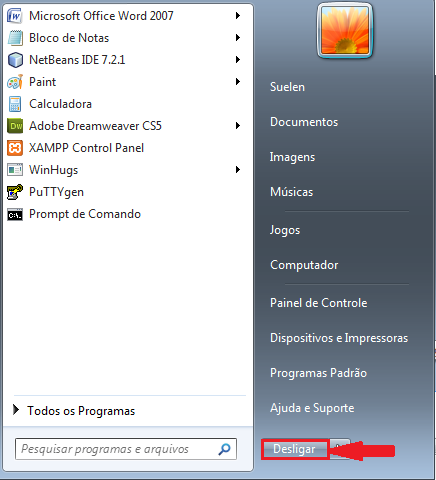
\includegraphics{Figures/desligando.png}
	\caption{Desligando o Computador}
	\label{Fig:desligando}
\end{figure}

\newpage

\section{O windows 7}

	
\end{document}